\newpage
\section{3次元気泡上昇流れ}

二層流の別のベンチマーク問題として3次元の気泡上昇流れ問題を解析し、参考文献の結果と比較した。

\subsection{解析条件}

Table \ref{table:3d-bubble-material-property}に二つの流体の物性値、Table \ref{table:3d-bubble-parameter}に解析パラメータを示す。
Case1は表面張力の影響が大きいケースであり、Case2は粘性の影響が大きいケースである。
ReとEoの値によって気泡の形が変わる分布を実験で分類している論文があり、Case1は球に近い形状を保った楕円形状であり、Case2では変形が大きくなる。

エトベス数$Eo = \rho g d^2 / \sigma$は、表面張力に対する重力の強さの指標。
ここで$d$は代表長さで気泡直径。(ボンド数Boとエトベス数Eoは同じ)


%ウェーバー数$We = \rho L U^2 / \sigma$は表面張力に対する慣性力の指標。
%\begin{figure}[H]
%	\centering
%	\includegraphics[width=6truecm]{pics/nond_number.png}
%	\caption{\cite{Himeno2023}}
%	\label{fig:3d-bubble-setting}
%\end{figure}

\renewcommand{\arraystretch}{1}
\begin{table}[H]
	\centering
	\caption{物性値}
	\begin{tabular}{cccccccccc}
		\hline
		Test case & $\rho_1$ & $\rho_2$ & $\mu_1$ & $\mu_2$ & $\mathrm{g}$ & $\sigma$ & $Eo (Bo)$ & $Re$ \\
		\hline 
		Case$1$ & $1000$ & $100$ & $10$ & $1$   & $0.98$ & $24.5$ & $10$ & $35$\\
		Case$2$ & $1000$ & $1$   & $10$ & $0.1$ & $0.98$ & $1.96$ & $125$ & $35$\\ 
		\hline         
	\end{tabular}
	\label{table:3d-bubble-material-property}
\end{table}
\renewcommand{\arraystretch}{1.0}

Case1は表面張力が強いため、数値安定性のために$\tau$を小さくする必要がある。\cite{Yamaguchi2018}
%表面張力の時間刻み制約は$\Delta t_{s} = \sqrt{(1000 + 100)\cdot \frac{10}{8 \pi}}\cdot 0.05^{\frac{3}{2}} = 0.234$

\renewcommand{\arraystretch}{1}
\begin{table}[H]
	\centering
	\caption{解析パラメータ}
	\begin{tabular}{cccccc}
		\hline
		Test case & $\Delta t$ & メッシュ幅$dx$ & 界面幅$D$ & 再初期化回数 & 再初期化$\Delta \tau$\\
		\hline 
		Case$1$ & $0.0025$ & $0.05$ & $0.04$ & $5$ & $0.001$\\
		Case$2$ & $0.0025$ & $0.05$ & $0.04$ & $5$ & $0.001$\\
		\hline         
	\end{tabular}
	\label{table:3d-bubble-parameter}
\end{table}
\renewcommand{\arraystretch}{1.0}

Figure \ref{fig:3d-bubble-setting}に文献\cite{Safi2017}から引用した解析領域の図を示す。

\begin{figure}[H]
	\centering
	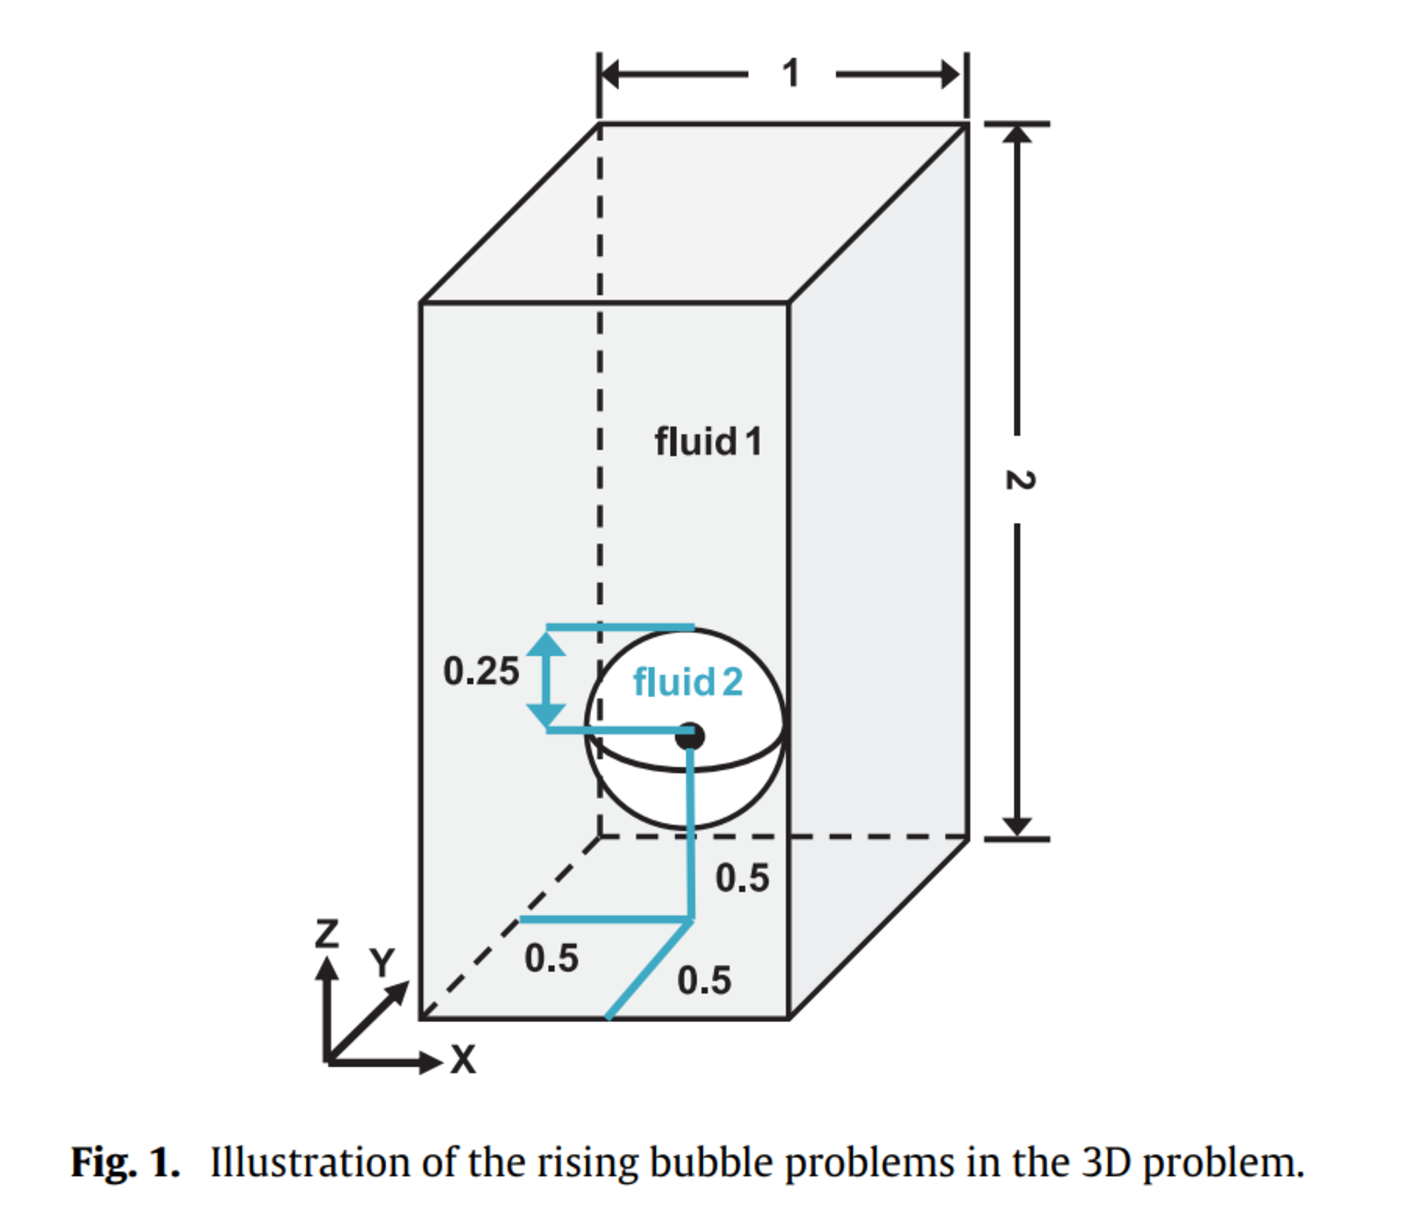
\includegraphics[width=10truecm]{pics/3d-bubble/setting.pdf}
	\caption{解析条件\cite{Safi2017}}
	\label{fig:3d-bubble-setting}
\end{figure}

Figure \ref{fig:3d-bubble-mesh}に解析用のメッシュを示す。メッシュは四面体$1$次要素を使用した。境界条件はダムブレイク問題と同様に上面を流出境界条件として圧力のディリクレ境界条件$p=0$、それ以外の面を滑りなし壁境界とした。
Figure \ref{fig:3d-bubble-levelset_t0_3d}に初期状態のレベルセット関数を示す。白い球面が界面である。

\begin{figure}[H]
	\centering
	\begin{minipage}[b]{0.49\columnwidth}
	    \centering
	    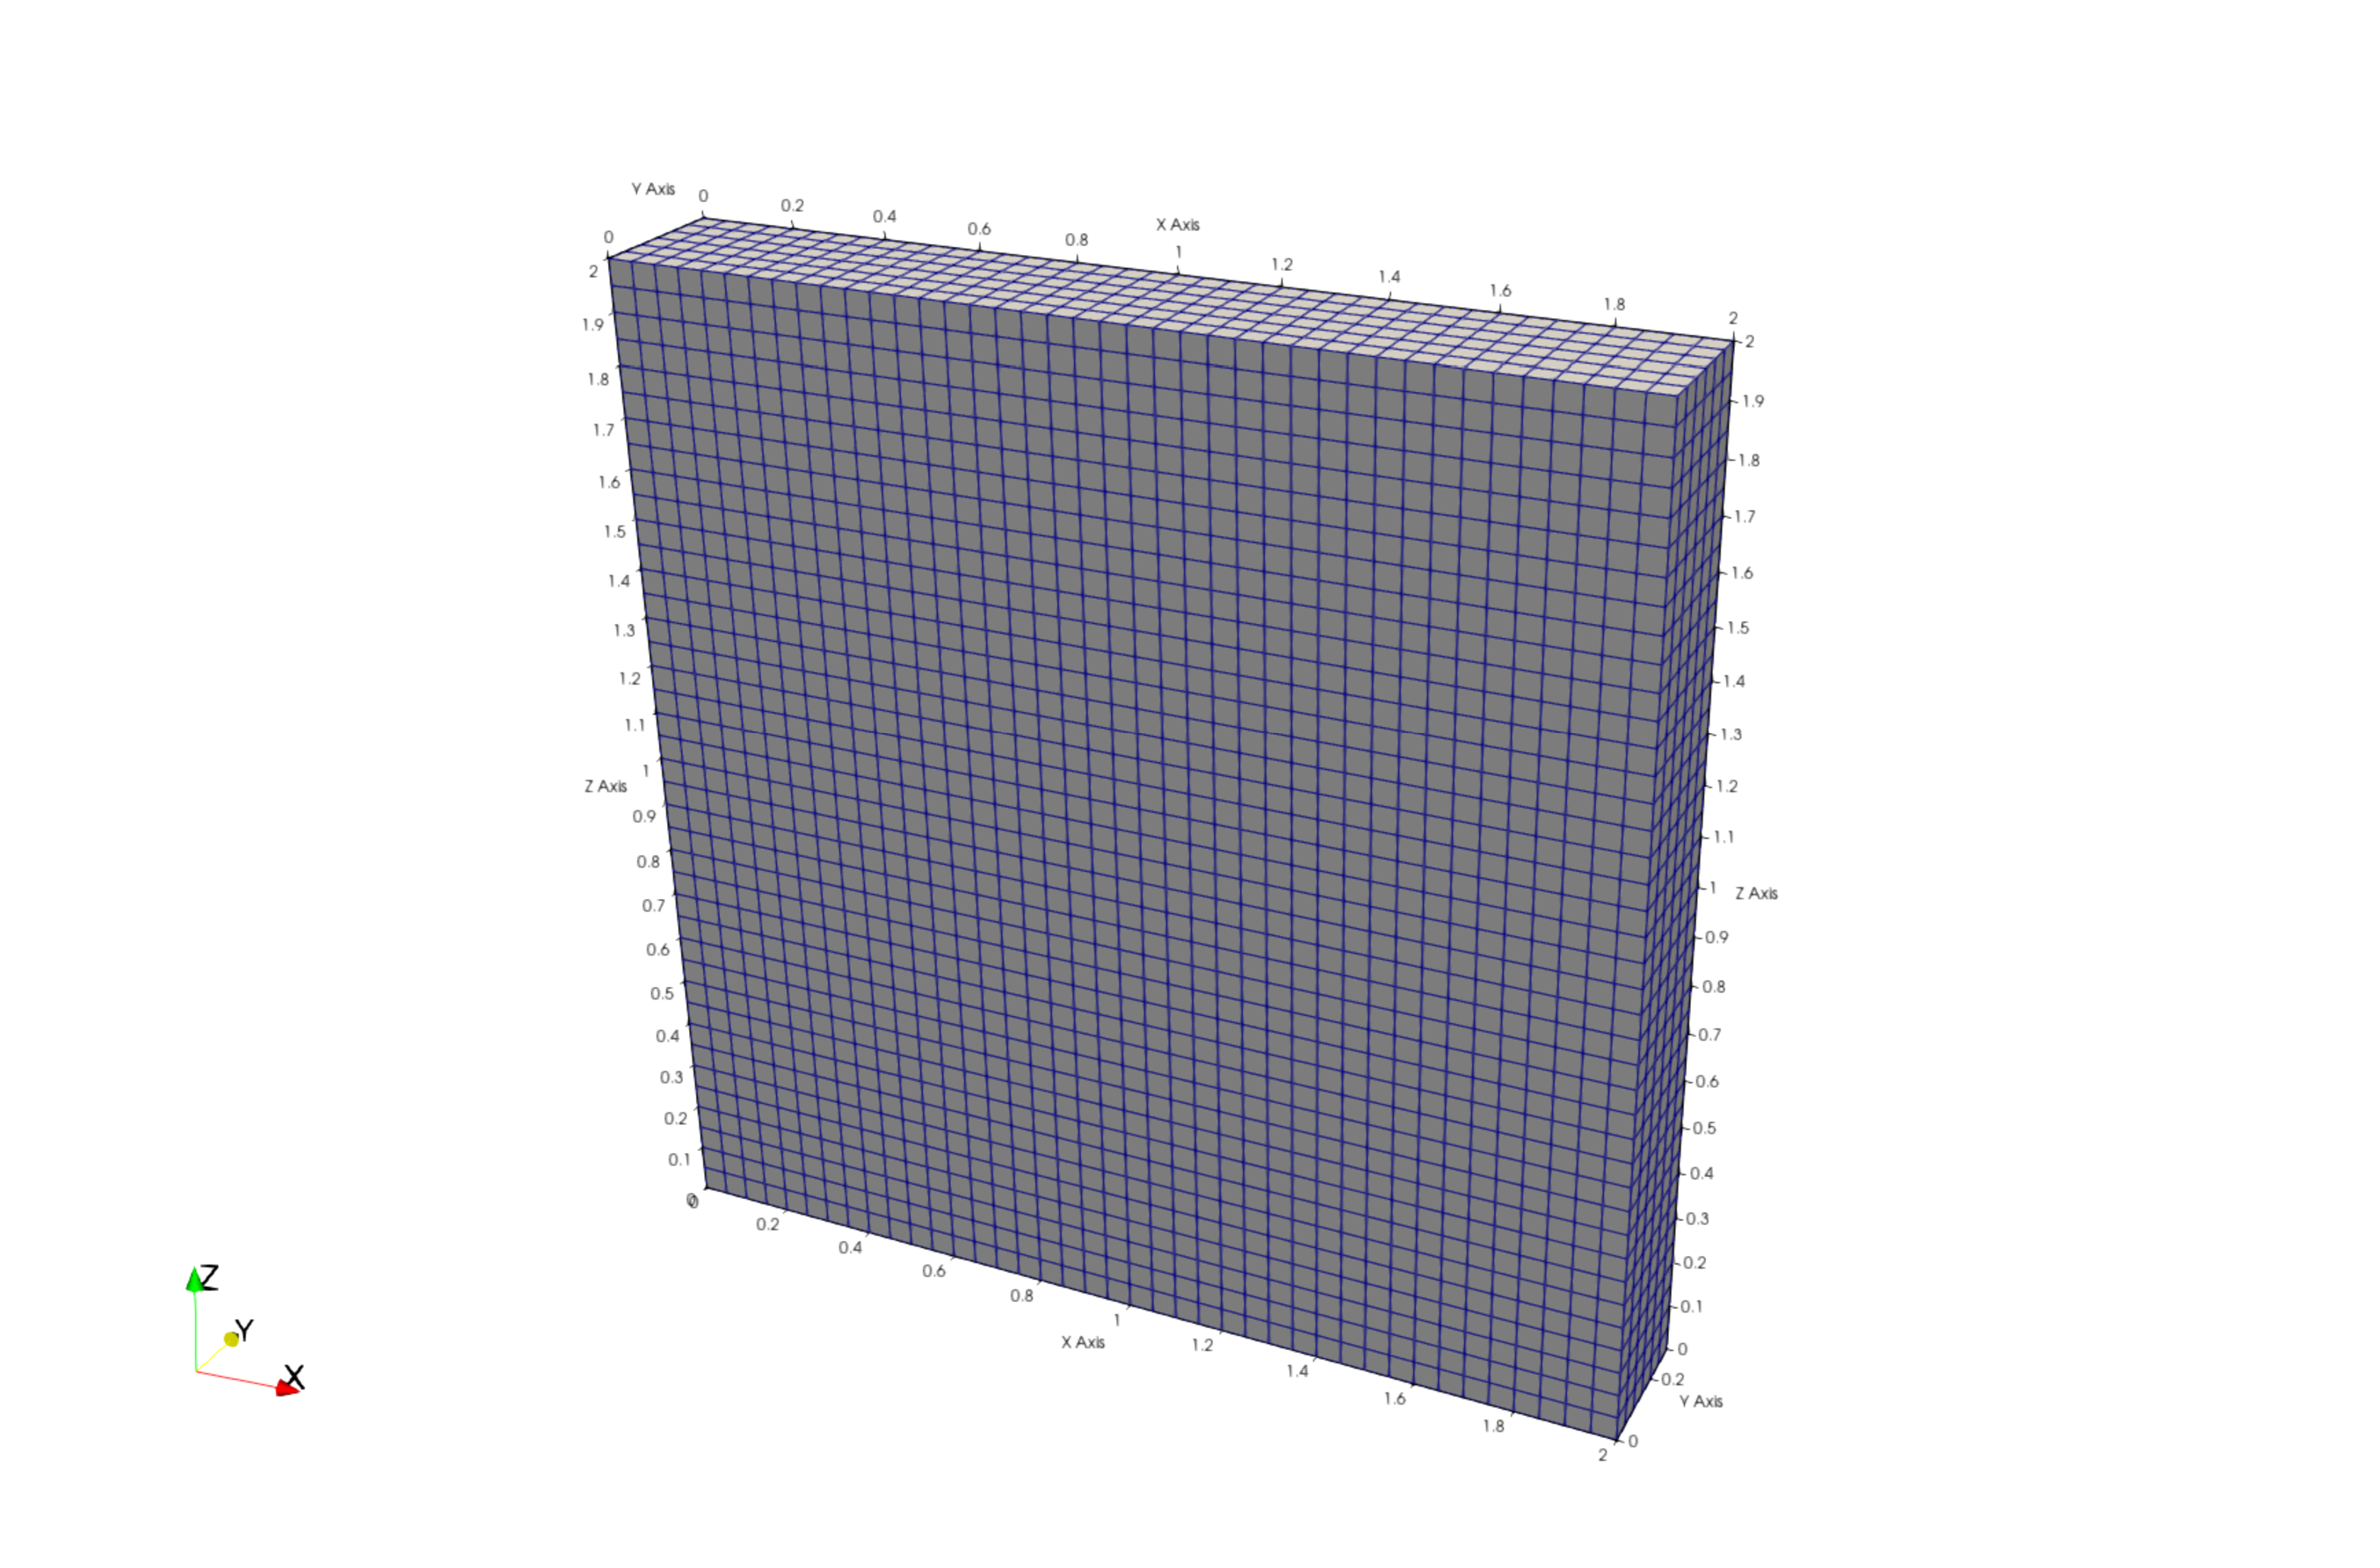
\includegraphics[width=6truecm]{pics/3d-bubble/mesh.jpeg}
		\caption{3次元気泡上昇流れの計算メッシュ}
		\label{fig:3d-bubble-mesh}
	\end{minipage}
	\begin{minipage}[b]{0.49\columnwidth}
	    \centering
	    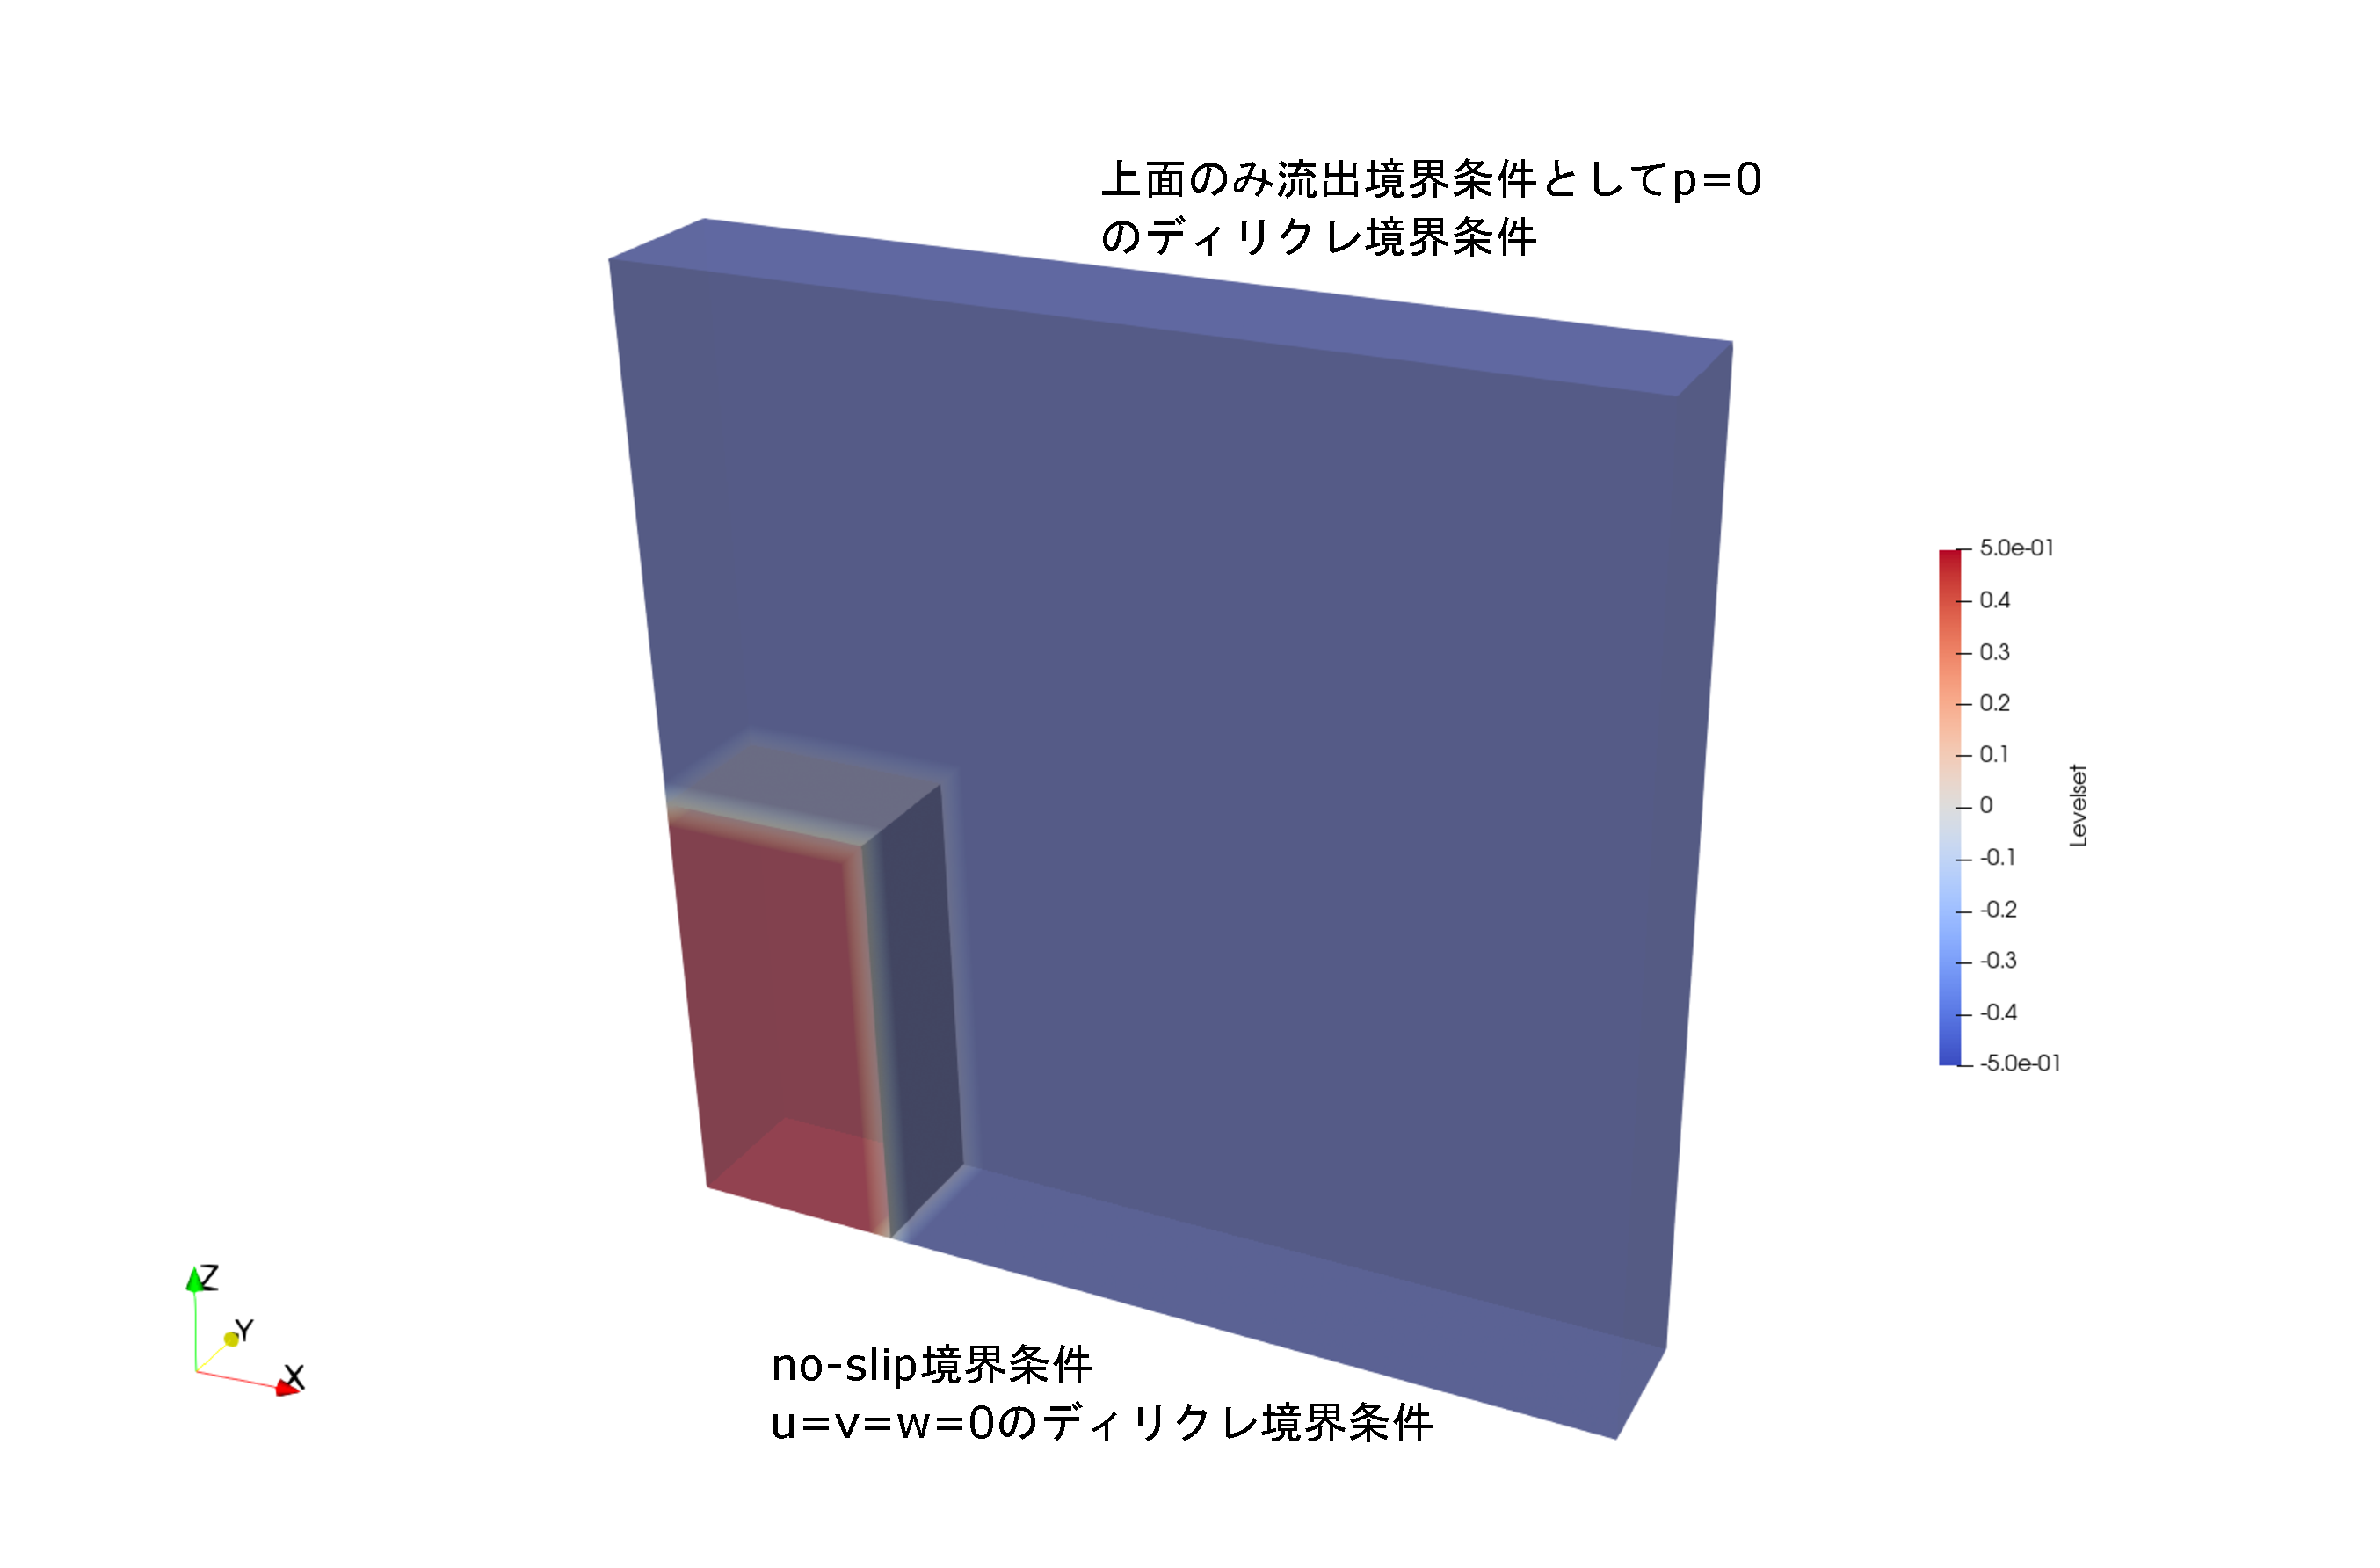
\includegraphics[width=6truecm]{pics/3d-bubble/levelset_init.jpeg}
		\caption{3次元気泡上昇流れのレベルセット関数($T=0$)}
		\label{fig:3d-bubble-levelset_t0_3d}
	\end{minipage}
\end{figure}

\newpage
\subsection{解析結果(Case1, 表面張力の影響が大きいケース)}
気泡上昇流れ問題においては表面張力の影響は大きいと思われるため、表面張力のモデルを導入し計算した結果を示す。

\begin{figure}[H]
	\centering
	\begin{minipage}[b]{0.16\columnwidth}
	    \centering
	    \includegraphics[width=3.3truecm]{pics/3d-bubble/tc1/result_0005.jpeg}
	\end{minipage}
	\begin{minipage}[b]{0.16\columnwidth}
	    \centering
	    \includegraphics[width=3.3truecm]{pics/3d-bubble/tc1/result_0015.jpeg}
	\end{minipage}
	\begin{minipage}[b]{0.16\columnwidth}
	    \centering
	    \includegraphics[width=3.3truecm]{pics/3d-bubble/tc1/result_0020.jpeg}
	\end{minipage}
	\begin{minipage}[b]{0.16\columnwidth}
	    \centering
	    \includegraphics[width=3.3truecm]{pics/3d-bubble/tc1/result_0025.jpeg}
	\end{minipage}
	\begin{minipage}[b]{0.16\columnwidth}
	    \centering
	    \includegraphics[width=3.3truecm]{pics/3d-bubble/tc1/result_0030.jpeg}
	\end{minipage}

	\caption{3次元気泡上昇流れのレベルセット関数の分布の時間変化(Case1, $\sigma=24.5$、表面張力あり、体積保存あり、再初期化あり)}
	\label{fig:3d-bubble_result_tc1}
\end{figure}

\begin{figure}[H]
    \centering
	\includegraphics[width=15truecm]{pics/3d-bubble/result-ref-tc1.png}
	\caption{参考文献結果(Case1)\cite{Safi2017}}
	\label{fig:3d-bubble-result-ref}
\end{figure}

\begin{figure}[H]
	\centering
	\begin{minipage}[b]{0.49\columnwidth}
	    \centering
	    \includegraphics[width=8truecm]{pics/3d-bubble/tc1_center.pdf}
		\caption{重心位置の時間変化(Case1)}
		\label{fig:3d-bubble-center-tc1}
	\end{minipage}
	\begin{minipage}[b]{0.49\columnwidth}
	    \centering
	    \includegraphics[width=8truecm]{pics/3d-bubble/tc1_velocity.pdf}
		\caption{上昇速度の時間変化(Case1)}
		\label{fig:3d-bubble-velocity-tc1}
	\end{minipage}
\end{figure}

\begin{comment}
\subsubsection{表面張力なしの解析結果}
\begin{figure}[H]
	\centering
	\begin{minipage}[b]{0.16\columnwidth}
	    \centering
	    \includegraphics[width=3.3truecm]{pics/3d-bubble/tc1-nosurfacetension/result_0005.jpeg}
	\end{minipage}
	\begin{minipage}[b]{0.16\columnwidth}
	    \centering
	    \includegraphics[width=3.3truecm]{pics/3d-bubble/tc1-nosurfacetension/result_0015.jpeg}
	\end{minipage}
	\begin{minipage}[b]{0.16\columnwidth}
	    \centering
	    \includegraphics[width=3.3truecm]{pics/3d-bubble/tc1-nosurfacetension/result_0020.jpeg}
	\end{minipage}
	\begin{minipage}[b]{0.16\columnwidth}
	    \centering
	    \includegraphics[width=3.3truecm]{pics/3d-bubble/tc1-nosurfacetension/result_0025.jpeg}
	\end{minipage}
	\begin{minipage}[b]{0.16\columnwidth}
	    \centering
	    \includegraphics[width=3.3truecm]{pics/3d-bubble/tc1-nosurfacetension/result_0029.jpeg}
	\end{minipage}

	\caption{3次元気泡上昇流れのレベルセット関数の分布の時間変化(Case1, $\sigma=0$、表面張力なし、体積保存あり、再初期化あり)}
	\label{fig:3d-bubble_result_tc1}
\end{figure}

\subsubsection{体積保存なしの解析結果}
\begin{figure}[H]
	\centering
	\begin{minipage}[b]{0.16\columnwidth}
	    \centering
	    \includegraphics[width=3.3truecm]{pics/3d-bubble/tc1-novolumecorrection/result_0005.jpeg}
	\end{minipage}
	\begin{minipage}[b]{0.16\columnwidth}
	    \centering
	    \includegraphics[width=3.3truecm]{pics/3d-bubble/tc1-novolumecorrection/result_0015.jpeg}
	\end{minipage}
	\begin{minipage}[b]{0.16\columnwidth}
	    \centering
	    \includegraphics[width=3.3truecm]{pics/3d-bubble/tc1-novolumecorrection/result_0020.jpeg}
	\end{minipage}
	\begin{minipage}[b]{0.16\columnwidth}
	    \centering
	    \includegraphics[width=3.3truecm]{pics/3d-bubble/tc1-novolumecorrection/result_0025.jpeg}
	\end{minipage}
	\begin{minipage}[b]{0.16\columnwidth}
	    \centering
	    \includegraphics[width=3.3truecm]{pics/3d-bubble/tc1-novolumecorrection/result_0030.jpeg}
	\end{minipage}

	\caption{3次元気泡上昇流れのレベルセット関数の分布の時間変化(Case1, $\sigma=24.5$、表面張力あり、体積保存なし、再初期化あり)}
	\label{fig:3d-bubble_result_tc1}
\end{figure}

\subsubsection{再初期化なしの解析結果}
\begin{figure}[H]
	\centering
	\begin{minipage}[b]{0.16\columnwidth}
	    \centering
	    \includegraphics[width=3.3truecm]{pics/3d-bubble/tc1-noreinitialization/result_0002.jpeg}
	\end{minipage}
	\begin{minipage}[b]{0.16\columnwidth}
	    \centering
	    \includegraphics[width=3.3truecm]{pics/3d-bubble/tc1-noreinitialization/result_0004.jpeg}
	\end{minipage}
	\begin{minipage}[b]{0.16\columnwidth}
	    \centering
	    \includegraphics[width=3.3truecm]{pics/3d-bubble/tc1-noreinitialization/result_0006.jpeg}
	\end{minipage}
	\begin{minipage}[b]{0.16\columnwidth}
	    \centering
	    \includegraphics[width=3.3truecm]{pics/3d-bubble/tc1-noreinitialization/result_0008.jpeg}
	\end{minipage}
	\begin{minipage}[b]{0.16\columnwidth}
	    \centering
	    \includegraphics[width=3.3truecm]{pics/3d-bubble/tc1-noreinitialization/result_0010.jpeg}
	\end{minipage}

	\caption{3次元気泡上昇流れのレベルセット関数の分布の時間変化(Case1, $\sigma=24.5$、表面張力あり、体積保存あり、再初期化なし)}
	\label{fig:3d-bubble_result_tc1}
\end{figure}
\end{comment}

\newpage
\subsection{解析結果(Case2, 表面張力の影響が小さいケース)}

\begin{figure}[H]
	\centering
	\begin{minipage}[b]{0.16\columnwidth}
	    \centering
	    \includegraphics[width=3.3truecm]{pics/3d-bubble/tc2/result_0005.jpeg}
	\end{minipage}
	\begin{minipage}[b]{0.16\columnwidth}
	    \centering
	    \includegraphics[width=3.3truecm]{pics/3d-bubble/tc2/result_0015.jpeg}
	\end{minipage}
	\begin{minipage}[b]{0.16\columnwidth}
	    \centering
	    \includegraphics[width=3.3truecm]{pics/3d-bubble/tc2/result_0020.jpeg}
	\end{minipage}
	\begin{minipage}[b]{0.16\columnwidth}
	    \centering
	    \includegraphics[width=3.3truecm]{pics/3d-bubble/tc2/result_0025.jpeg}
	\end{minipage}
	\begin{minipage}[b]{0.16\columnwidth}
	    \centering
	    \includegraphics[width=3.3truecm]{pics/3d-bubble/tc2/result_0030.jpeg}
	\end{minipage}

	\caption{3次元気泡上昇流れのレベルセット関数の分布の時間変化(Case2, $\sigma=1.95$、表面張力あり、界面幅$D=0.10$)}
	\label{fig:3d-bubble_result_tc2}
\end{figure}

\begin{figure}[H]
    \centering
	\includegraphics[width=15truecm]{pics/3d-bubble/result-ref-tc2.png}
	\caption{参考文献結果(Case2)\cite{Safi2017}}
	\label{fig:3d-bubble-result-ref}
\end{figure}

\begin{figure}[H]
	\centering
	\begin{minipage}[b]{0.49\columnwidth}
	    \centering
	    \includegraphics[width=8truecm]{pics/3d-bubble/tc2_center.pdf}
		\caption{重心位置の時間変化(Case2)}
		\label{fig:3d-bubble-center-tc2}
	\end{minipage}
	\begin{minipage}[b]{0.49\columnwidth}
	    \centering
	    \includegraphics[width=8truecm]{pics/3d-bubble/tc2_velocity.pdf}
		\caption{上昇速度の時間変化(Case2)}
		\label{fig:3d-bubble-velocity-tc2}
	\end{minipage}
\end{figure}

\newpage
\subsection{解析結果(並列化計算)}

領域分割法による並列計算結果についても検証を行った。
図~\ref{fig:3d-bubble-mesh-parallel16}に領域分割数16の場合の計算メッシュの分割結果を示す。
節点数は34476, 要素数は31250である。

\begin{figure}[H]
    \centering
    \includegraphics[width=6truecm]{pics/3d-bubble-parallel/mesh_parallel16.jpeg}
	\caption{3次元気泡上昇流れの計算メッシュ(領域分割数16の場合)}
	\label{fig:3d-bubble-mesh-parallel16}
\end{figure}

図~\ref{fig:3d-bubble-center-tc1-parallel}~~\ref{fig:3d-bubble-velocity-tc2-parallel}に並列数2,4, 8, 16の場合の計算結果を示す。
並列数を変えた場合でも逐次計算の結果と一致した結果が得られた。

\begin{figure}[H]
	\centering
	\begin{minipage}[b]{0.49\columnwidth}
	    \centering
	    \includegraphics[width=8truecm]{pics/3d-bubble-parallel/tc1_center_parallel_comparison.pdf}
		\caption{重心位置の時間変化の並列数による比較(Case1)}
		\label{fig:3d-bubble-center-tc1-parallel}
	\end{minipage}
	\begin{minipage}[b]{0.49\columnwidth}
	    \centering
	    \includegraphics[width=8truecm]{pics/3d-bubble-parallel/tc1_velocity_parallel_comparison.pdf}
		\caption{上昇速度の時間変化の並列数による比較(Case1)}
		\label{fig:3d-bubble-velocity-tc1-parallel}
	\end{minipage}
\end{figure}

\begin{figure}[H]
	\centering
	\begin{minipage}[b]{0.49\columnwidth}
	    \centering
	    \includegraphics[width=8truecm]{pics/3d-bubble-parallel/tc2_center_parallel_comparison.pdf}
		\caption{重心位置の時間変化の並列数による比較(Case2)}
		\label{fig:3d-bubble-center-tc2-parallel}
	\end{minipage}
	\begin{minipage}[b]{0.49\columnwidth}
	    \centering
	    \includegraphics[width=8truecm]{pics/3d-bubble-parallel/tc2_velocity_parallel_comparison.pdf}
		\caption{上昇速度の時間変化の並列数による比較(Case2)}
		\label{fig:3d-bubble-velocity-tc2-parallel}
	\end{minipage}
\end{figure}

図~\ref{fig:3d-sloshing-parallel-speedup}に並列化による加速率効率のグラフを示す。
\begin{figure}[H]
    \centering
	\includegraphics[width=15truecm]{pics/3d-bubble-parallel/bubble_parallel_speedup.jpg}
	\caption{気泡上昇解析の並列化効率}
	\label{fig:3d-bubble-parallel-speedup}
\end{figure}